%!TEX root = ../article.tex

\subsection{Fusion categories and fields of definition}
Let $k$ be a field.  An object in an additive category is called simple if it has no non-trivial proper subobjects.  An additive category is called semisimple if every object is a direct sum of simple objects (and in particular, every indecomposable object is simple).  A category is called idempotent complete (or Karoubian or psuedoabelian) if every idempotent has an image (that is, a subobject which the idempotent factors through).  It is easy to see that any idempotent complete additive semisimple category is abelian.  A \emph{split semisimple category over $k$} is a semisimple category over $k$ such that every simple object $X$ is split simple, that is $\End{X} = k$.  If $k$ is an algebraically closed field, then any semisimple category over $k$ is automatically split.

A \emph{fusion category over $k$} is a $k$-linear abelian semisimple rigid monoidal category with finitely many isomorphism classes of simple objects.  A \emph{split fusion category over $k$} is a fusion category over $k$ which is split semisimple.  (Warning, some authors require that all fusion categories be split.)

\begin{example}
Consider $\Real[\Integer/3 \Integer]\text{-mod}$.   This is a fusion category  over $\Real$ with two objects: the trivial module and the $2$-dimensional representation (where the generator acts by $120$-degree rotation).  It is not split fusion because the endomorphism algebra of the $2$-dimensional representation is $\Complex$.
\end{example}

Suppose that $k<K$ is an inclusion of fields and that $\cC_K$ is a semisimple abelian category over $K$ possibly with some fixed additional structures (e.g. it's a monoidal rigid category or a braided category).  A \emph{rational form} of $\cC$ over $k$ is a semisimple abelian category $\cC_k$ over $k$ (again with the same structure) together with an equivalence between the idempotent completion of $\cC_k \otimes_k K$ is and $\cC_K$ (this equivalence should preserve the additional structure).  A \emph{complete rational form} of $\cC$ over $k$ is a rational form $\cC_k$ such that $\cC_k \otimes_k K \cong \cC_K$, in other words, a complete rational form is a rational form such that $\cC_k \otimes_k K$ is already idempotent complete.

%Suppose that $k<K$ is an inclusion of fields and suppose that $\cC_K$ is a semisimple abelian tensor category over $K$.  A \emph{rational form} of $\cC$ over $k$ is a fusion category $\cC_k$ over $k$ such that the idempotent additive completion of $\cC_k \otimes_k K$ is equivalent to $\cC_K$.  A \emph{complete rational form} of $\cC$ over $k$ is a fusion category $\cC_k$ such that $\cC_k \otimes_k K \cong \cC_K$, in other words, a complete rational form is a rational form such that $\cC_k \otimes_k K$ is already idempotent complete.

There are several reasons for considering incomplete rational forms.  First, many constructions do not preserve completeness.  For example, the category of $G$-graded rational vector spaces is a complete rational form of the category of $G$-graded complex vector spaces, while the center of the former category is only an incomplete rational form of the center of the latter.  Second, any fusion category is the category of representations of a weak Hopf algebra $A$ \cite{MR1976459, 0206113, 9904073, MR2522429} and if that weak Hopf algebra has an rational form $A_k$ then $A_k-\text{mod}$ is, in general, an incomplete rational form for $A-\text{mod}$.  Third, the notion of incomplete rational form arises naturally in the context of planar algebras.  Finally, it can be convenient to show that $\cC_k$ is a complete rational form by first showing that it is a rational form (which is often easy for the above reasons) and then explicitly checking completeness.

Notice that if $\cC_K$ is a split fusion category over $K$ and $\cC_k$ is a rational form over $k < K$ then $\cC_k$ is complete if and only if $\cC_k$ is a split fusion category.

%A \emph{split rational form} is a rational form $\cC_k$ which is a split.  We say that $\cC_K$ is \emph{defined over} $k$ if there exists a split rational form $\cC_k$.  We will be interested in the case $K = \Complex$ and $k$ a number field.  An important equivalent condition to $\cC_k$ being split is that base extension give an isomorphism on Grothendieck groups $K_0(\cC_k) \cong K_0(\cC_K)$.  In particular, any rational form for $\cC_K$ categorifies the same fusion ring.

If $\cC_K$ is a split fusion category then there is a more concrete description of having a complete rational form (pointed out to us by Victor Ostrik).  A split fusion category $\cC_K$ can be completely described by a collection of vector spaces $\Hom{}{V_a \otimes V_b}{V_c}$ over $K$, and associativity maps between the appropriate tensor products of these spaces.   The fusion category $\cC_K$ has a complete rational form over $k$ if and only if there exists a basis for each of these vector spaces such that all the associativity maps are given by matrices with entries in $k$.

\begin{example} \label{ex:graded}
$\cC_\Complex = \Complex[\Integer/3 \Integer]\text{-mod}$ has a complete rational form over $\Rational$.  To see this notice that $\Integer/3\Integer$ is abelian, and hence $\Complex[\Integer/3 \Integer]\text{-mod}$ is equivalent to the category of $\Integer/3 \Integer$-graded complex vector spaces.  We can take $\cC_\Rational$ to be the category of $\Integer/3 \Integer$-graded rational vector spaces.
\end{example}

\begin{example} \label{ex:incomplete}
Consider $G$ a finite group.  Notice that all of the representations of a group $G$ are defined over a field $k$ if and only if $k[G]\text{-mod}$ is split.  All representations of any finite group $G$ are defined over $\Rational(\zeta_{n})$, where $n$ is the exponent of $G$.  Therefore, $\Complex[G]\text{-mod}$ has a complete rational form over a cyclotomic field.  On the other hand as Example \ref{ex:graded} shows, it is possible for $\Complex[G]\text{-mod}$ to be defined over a smaller field than the minimal field of definition for all its representations.
\end{example}

If $\cC$ is a $k$-linear category, and $k < K$ is an inclusion of fields and the idempotent additive completion of $\cC \tensor_k K$ is semisimple, then $\cC$ is semisimple.  This follows from the characterization of semisimplicity in terms of semisimplicity of the endomorphism algebras, given in the next Lemma, and the equivalence of semisimplicity of artinian rings with the absence of nilpotent ideals \cite[p. 203]{MR1009787}.  The same is not true for split semisimplicity as  $\Real[\Integer/3 \Integer]\text{-mod}$ is not split semisimple while  $\Complex[\Integer/3 \Integer]\text{-mod}$ is.  The converse is also false at least when $k<K$ is inseparable \cite[Question 5.1]{MR1995781}.


\begin{lem}
A $k$-linear additive idempotent complete category $\cC$ is semisimple if and only if the endomorphism algebra of every object is a semisimple algebra.  The simple objects are exactly those objects whose endomorphism algebras are division rings.
\end{lem}
\begin{proof}
By Schur's lemma, if $\cC$ is semisimple then the endomorphism algebra of an object is a sum of matrix algebras over division rings, which is a semisimple algebra.

In the other direction, suppose that $\cC$ has all endomorphism algebras semisimple.  Since the category is idempotent complete, one may use the projections in the endomorphism algebras to decompose any object into a direct sum of objects whose endomorphism algebras are division rings.  If $X$ and $Y$ are non-isomorphic objects whose endomorphism algebras are division rings, the semisimplicity of $\End{X\oplus Y}$ shows that there are no nonzero maps between $X$ and $Y$.  Hence all objects whose endomorphism algebras are division rings are simple and every object is semisimple.
\end{proof}


%If $k<\Complex$ and $\cC$ is a fusion category over $\Complex$ then a \emph{rational form} of $\cC$ over $k$ is a fusion category $\cC_k$ over $k$ such that $\cC_k \otimes_k \Complex \cong \cC$ and such that the Grothendieck group $K_0(\cC_k) = K_0(\cC)$ (or equivalently such that every simple object in $\cC_k$ is absolutely simple). The latter condition is necessary in order for this concept to match up with field of definition of representations of algebras, for example even though the representation theory of $\Integer/3\Integer$ is not defined over $\Real$ nonetheless $\Real[\Integer/3\Integer]\text{-mod} \otimes_\Real \Complex \cong \Complex[\Integer/3\Integer]\text{-mod}$. \scott{Clunky sentence} In particular with our terminology $\Complex[\Integer/3\Integer]\text{-mod}$ does not have a rational form over $\Real$.  If $\cC$ has a rational form over $k$ we say that $\cC$ is \emph{defined over} $k$.

\subsection{Subfactors and category theory}

The main examples in this paper come from the theory of subfactors.  A subfactor is an inclusion $A \subset B$ of von Neumann algebras with trivial centers.  The applications of subfactor theory to tensor categories involve subfactors of finite index.

From such a subfactor $A \subset B$, we can construct a pair of $\Complex$-linear abelian semisimple rigid tensor categories (that is, categories that only fail to be fusion categories by possibly having infinitely many non-isomorphic simple objects).  See \cite{MR1424954} for more details. These tensor categories are  the subcategory of the category of $A\text{-}A$ bimodules tensor generated by ${}_A B_A$ and the subcategory of $B\text{-}B$ bimodules tensor generated by ${}_B B_A \otimes_A {}_A B_B$.  These tensor categories are fusion if and only if the subfactor is finite depth.

It will not be important to this paper to understand subfactors or their bimodules. Although our main examples come from subfactors, these subfactors can be constructed via their planar algebras, and we can define the two associated tensor categories directly from the planar algebra.

\subsection{Shaded planar algebras}

One of the main tools for understanding monoidal categories (and more generally $2$-categories) is the diagram calculus (pioneered by Penrose \cite{MR0281657}, Joyal-Street \cite{MR1113284}, Reshetikhin-Turaev \cite{MR1036112}, etc.) of string diagrams.  Planar algebras are a version of this diagram calculus which allows you to study monoidal categories from the point of view of a particular object, where you only consider strings labelled by that object.

In particular, given a subfactor the resulting string diagrams have regions which are checkerboard shaded (corresponding to $A$ and $B$) and unoriented unlabelled strings (depending on the shading this string represents either ${}_A B_B$ or ${}_B B_A$).  The structure here is a called a ``shaded planar algebra."

We sketch the definition here.  For further details, see  \cite[\S 2]{MR1865703}, \cite[\S 0]{math.QA/9909027}, or \cite{MR1957084}.
%(The original definition is phrased in terms of colored operads, but essentially the same).

\begin{defn}
A {\em (shaded) planar tangle} 
has an outer disk,
a finite number of inner disks,
and a finite number of non-intersecting strings.
A string can be either a closed loop
or an edge with endpoints on boundary circles.
We require that
there be an even number of endpoints on each boundary circle,
and a checkerboard shading of
the regions in the complement of the interior disks.
We further require that there be a marked point on the boundary of each disk, and that the inner disks are ordered.

Two planar tangles are considered equal if they are isotopic (not necessarily rel boundary).

Here is an example of a planar tangle.
$$\inputtikz{SampleTangle}$$

Planar tangles can be composed by placing one planar tangle inside an interior disk of another,
lining up the marked points,
and connecting endpoints of strands.
The numbers of endpoints and the shadings must match up appropriately.  This composition turns the collection of planar tangles into a colored operad.
\end{defn}

\begin{defn}
A {\em (shaded) planar algebra} over a field $k$ consists of
\begin{itemize}
\item A family of vector spaces $\{V_{(n,\pm,)}\}_{n\in \Natural}$ over $k$, called the positive and negative $n$-box spaces.
\item For each planar tangle, a multilinear map $V_{n_1, \pm_1} \otimes \ldots \otimes V_{n_j, \pm_j} \rightarrow V_{n_0, \pm_0}$ where $n_i$ is half the number of endpoints on the $i$th interior boundary circle, $n_0$ is half the number of endpoints on the outer boundary circle, and the signs $\pm$ are positive (respectively negative) when the marked point on the corresponding boundary circle is in an unshaded (respectively shaded) region.
\end{itemize}

For example, the planar tangle above gives a map $$V_{1,+} \otimes V_{2,+} \otimes V_{2,-} \rightarrow V_{3,+}.$$

The linear map associated to a `radial' tangle (with one inner disc, radial strings, and matching marked points) must be the identity.
We require that the action of planar tangles be compatible with composition of planar tangles.  In other words, composition of planar tangles must correspond to the obvious composition of multilinear maps.  \end{defn}

We will refer to an element of $V_{n,\pm}$ (and specifically $V_{n,+}$, unless otherwise stated) as an ``$n$-box.''

We make frequent use of three families of planar tangles
called multiplication, trace, and tensor product, which are shown in Figure \ref{fig:timestracetensor}.
``Multiplication'' gives an associative product
$V_{n,\pm} \otimes V_{n,\pm} \rightarrow V_{n,\pm}$.
``Trace'' gives a map $V_{n,\pm} \rightarrow V_{0,\pm}$.
``Tensor product'' gives an associative product
$V_{m,\pm} \otimes V_{n,\pm} \rightarrow V_{m+n,\pm}$ if $m$ is even,
or $V_{m,\pm} \otimes V_{n,\mp} \rightarrow V_{m+n,\pm}$ if $m$ is odd.

\begin{figure}[ht]
$$\inputtikz{multiplication} \quad , \quad \inputtikz{trace} \quad , \quad \inputtikz{tensor}$$
\caption
  {The multiplication, trace, and tensor product tangles.}
\label{fig:timestracetensor}
\end{figure}

The (shaded or unshaded) empty diagrams can be thought of as elements of $V_{0,\pm}$, since the `empty tangle' induces a map from the empty tensor product $\Complex $ to the space $V_{0,\pm}$.  If the space $V_{0,\pm}$ is one dimensional
then we can identify it with $\Complex$  by sending the empty diagram to one.

%\begin{defn}
%A planar algebra is called simple if $\dim V_{0,\pm} = 1$.
%\end{defn}

\begin{defn}
A planar algebra is called \emph{irreducible} if $\dim V_{0,\pm} = 1$ and $\dim V_{1,\pm} = 1$.
\end{defn}

\begin{defn}\label{defn:uncappable}
An $n$-box $S$ is {\em uncappable}  if $\epsilon_i(S)=0$ for all $i=1,\cdots, 2n$ where
 $$\epsilon_1 = \inputtikz{epsilon1} \, , \qquad 
 \epsilon_2 = \inputtikz{epsilon2} \, , \quad \ldots , \qquad 
 \epsilon_{2n}= \inputtikz{epsilon2k} \, . $$
 
 We say $S$ is a {\em rotational eigenvector with eigenvalue $\omega$} if   $\rho(S)= \omega S$ where
  $$\rho=\inputtikz{rho} \, .$$
 Note that $\omega$ must be a $n^{th}$ root of unity.
\end{defn}

Given a shaded planar algebra we can recover two tensor categories called its even parts.  However to describe this we need to deal with an annoying technical point.  Recall that the planar algebra only captures maps between tensor products of a fixed generating object.  If every object of a semisimple tensor category appears as a summand of some tensor power of a fixed object, then the tensor category can be recovered from the full subcategory of these tensor powers by taking the idempotent completion.

\begin{defn}
The idempotent completion of a tensor category $\check{\cC}$ is a tensor category $\cC$ which contains $\check{\cC}$ as a full sub-category. The objects of $\cC$ are pairs $(o,p)$, where $o$ is an object of $\check{\cC}$ and $p:o \to o$ is an idempotent in $\check{\cC}$.  We define $$\Hom{\cC}{(o,p)}{(o',p')} = \setcl{ f \in \Hom{\check{\cC}}{o}{o'} }{ f p = f = p' f}$$ and inherit composition and tensor product.  (When we say $\check{\cC}$ is a full sub-category of $\cC$ we are implicitly identifying $o$ with $(o,\id_o)$.)
\end{defn}


\begin{defn}
If $\cP$ is a shaded planar algebra, let $\check{\cP}^p$ be the category whose objects are even integers and whose morphisms are given by
$$\Hom{\check{\cP}^p}{2m}{2n} = V_{m+n,+}.$$
 Let $\cP^p$, called the principal even part of $\cP$ be the idempotent completion of the additive completion of $\check{\cP}^p$.

Similarly define $\check{\cP}^d$ whose objects are even integers and whose morphisms are given by
$$\Hom{\check{\cP}^d}{2m}{2n} = V_{m+n,-},$$ and the dual even part $\cP^d$ to be the idempotent completion of the additive completion of $\check{\cP}^d$.
\end{defn}

A planar algebra is called \emph{unitary} if there is an antilinear adjoint operation $*$ on each $V_{n,\pm}$, compatible with the adjoint operation on planar tangles given by reflection such that the sesquilinear form $\langle x,y \rangle = \tr{x y^*}$ is positive definite.  The even parts of a unitary planar algebra are semisimple because all the endomorphism algebras are finite dimensional $\Complex^*$ algebras which are necessarily semisimple.  Often in order to construct a unitary planar algebra from a non-unitary planar algebra we quotient out by the radical of $\langle x,y \rangle = \tr{x y^*}$, which is called the ideal of negligible morphisms.

Suppose that $k<K$ is an inclusion of fields and suppose that $\cP$ is a planar algebra over $K$.  A \emph{rational form} of $\cP$ over $k$ is a planar algebra $\cP_k$ over $k$ such that $\cP_k \otimes_k K$ is isomorphic to $\cP$.  If $\cP_k$ is a rational form for $\cP$ then the corresponding fusion categories $\cP_k^p$ and $\cP_k^d$ are rational forms for $\cP^p$ and $\cP^d$.  The rational form $\cP_k^p$ is a complete rational form for $\cP^p$ if every isomorphism class of projection in $V_{m+n,+}(\cP)$ has a representative coming from $V_{m+n,+}(\cP^p)$ (and similarly for the dual even part).

\subsection{Principal graphs}

Given a unitary irreducible shaded planar algebra $\cP$ the principal graphs are a pair of bipartite graphs which together encode the fusion rules for tensoring with the single strand.

The principal graph has even vertices corresponding to isomorphism classes of simple projections in $V_{\text{even},+}$ and odd vertices corresponding to the isomorphism classes of simple projections in $V_{\text{odd},+}$.  An even vertex $V$ and an odd vertex $W$ are connected by $\dim \Hom{}{W \otimes X}{V}$ edges, where $X$ is the single strand.  The dual principal graph has even vertices corresponding to isomorphism classes of simple projections in $V_{\text{even},-}$, odd vertices corresponding $V_{\text{odd},-}$, and edges given by the fusion with the single strand of the opposite shading.

A subfactor is called \emph{finite depth} if the principal graph is finite.

\subsection{The lopsided normalization}
\label{sec:lopsided}%
In an irreducible shaded planar algebra $\cP$ over a field $k$, the shaded inside and shaded outside circles each evaluate to a scalar multiple of the empty diagram. These multiples are called the shaded and unshaded moduli. The product of the two moduli is called the index of $\cP$.

If the two moduli are equal, we say the planar algebra is spherical. (In particular, because in this section we are assuming irreducibility, this condition implies the usual notion of a planar algebra being spherical.) If the shaded modulus is equal to one, we say the planar algebra is lopsided, and the unshaded modulus is the index.

Any irreducible shaded planar algebra $\cP$ over $\Complex$ is part of a family $\left\{\cP_x\right\}_{x \in \Complex}$ of planar algebras with $\cP_1 = \cP$, and $\cP_x$ given by changing the action of the planar operad by a factor of $x^k$, where $k$ is the signed count of critical points in the strands which are shaded above and unshaded below (minima counting positively, maxima counting negatively). The index is constant across this family, but the shaded and unshaded moduli scale by $x$ and $x^{-1}$. 

It may be that the planar algebra $\cP_x$ has a rational form over a field $k$ for certain $x$, but not all $x$.  In particular, given a planar algebra $\cC$ over $k$ with unshaded modulus $x \in k$, then $\cC_{x^{-1}}$ is a lopsided planar algebra over $k(x)=k$.  On the other hand, given a lopsided planar algebra $\cC$ over $k$ with index $D \in k$ the corresponding spherical planar algebra $\cC_{\sqrt{D}}$ is in general only defined over $k(\sqrt{D})$.  The fact that the field of definition may need to increase to ensure being spherical but does not need to increase to ensure being lopsided should encourage you to prefer lopsided planar algebras over spherical planar algebras. (It's also natural from a subfactor perspective: $B$ as an $A-B$ bimodule has left-dimension the index and right-dimension $1$.)

\newcommand{\trl}[1]{\operatorname{tr}_{L}\left(#1\right)}
\newcommand{\trr}[1]{\operatorname{tr}_{R}\left(#1\right)}

Any element $v \in \cP_{n,\pm}$ has a left trace and a right trace, satisfying
\begin{align*}
\trl{v} & =
	\begin{cases}
		\trr{v} & \text{if $n$ is even} \\
		\frac{d_{\mp}}{d_{\pm}} \trr{v} & \text{if $n$ is odd}
	\end{cases}
\end{align*}
where $d_+$ is the unshaded modulus and $d_-$ is the shaded modulus. When $\cP$ is spherical, the left and right traces coincide. We will sometimes refer to the trace of an idempotent as its dimension, and if a side is not specified we always intend the right trace.

\begin{example}
The two strand Jones-Wenzl idempotents in lopsided Temperley-Lieb are 
\begin{align*}
\begin{tikzpicture}[baseline=-1ex]
\node[fill=white, draw, rectangle] (left) at (0,0) {$\JW{2}$};
\begin{pgfonlayer}{background} 
\path[fill=black!20]
	($(left.240)+(0,-0.5)$) -- ($(left.120)+(0,0.5)$) -- ($(left.60)+(0,0.5)$) -- ($(left.300)+(0,-0.5)$);
\draw ($(left.240)+(0,-0.5)$) -- ($(left.120)+(0,0.5)$);
\draw  ($(left.60)+(0,0.5)$) -- ($(left.300)+(0,-0.5)$);
\end{pgfonlayer}
\end{tikzpicture}
& = 
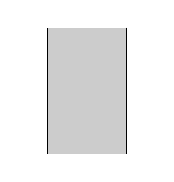
\begin{tikzpicture}[baseline=-1ex]
\clip (-0.75,-0.8) rectangle (0.75,0.8);
\path[fill=black!20]
	 (-0.5,-0.8) -- (-0.5,0.8) -- (0.5,0.8) -- (0.5,-0.8);
\draw (-0.5,-0.8) -- (-0.5,0.8);
\draw  (0.5,0.8) -- (0.5,-0.8);
\end{tikzpicture}
 - 
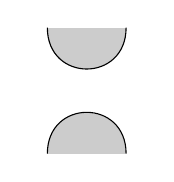
\begin{tikzpicture}[baseline=-1ex]
\clip (-0.75,-0.8) rectangle (0.75,0.8);
\path[draw, fill=black!20]
	 (-0.5,-0.8) .. controls ++(0,0.7) and ++(0,0.7) .. (0.5,-0.8);
\path[draw, fill=black!20]
	 (-0.5,0.8) .. controls ++(0,-0.7) and ++(0,-0.7) .. (0.5,0.8);
\end{tikzpicture}
\displaybreak[1] \\
\intertext{and}
\begin{tikzpicture}[baseline=-1ex]
\node[fill=white, draw, rectangle] (left) at (0,0) {$\JW{2}$};
\begin{pgfonlayer}{background} 
\path[fill=black!20] (-0.75,-0.8) rectangle (0.75,0.8);
\path[fill=white]
	($(left.240)+(0,-0.5)$) -- ($(left.120)+(0,0.5)$) -- ($(left.60)+(0,0.5)$) -- ($(left.300)+(0,-0.5)$);
\draw ($(left.240)+(0,-0.5)$) -- ($(left.120)+(0,0.5)$);
\draw  ($(left.60)+(0,0.5)$) -- ($(left.300)+(0,-0.5)$);
\end{pgfonlayer}
\end{tikzpicture}
& = 
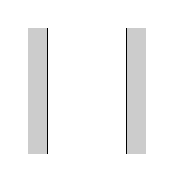
\begin{tikzpicture}[baseline=-1ex]
\path[fill=black!20] (-0.75,-0.8) rectangle (0.75,0.8);
\path[fill=white]
	 (-0.5,-0.8) -- (-0.5,0.8) -- (0.5,0.8) -- (0.5,-0.8);
\draw (-0.5,-0.8) -- (-0.5,0.8);
\draw  (0.5,0.8) -- (0.5,-0.8);
\end{tikzpicture}
 -  \frac{1}{[2]^2}
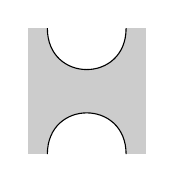
\begin{tikzpicture}[baseline=-1ex]
\path[fill=black!20] (-0.75,-0.8) rectangle (0.75,0.8);
\path[draw, fill=white]
	 (-0.5,-0.8) .. controls ++(0,0.7) and ++(0,0.7) .. (0.5,-0.8);
\path[draw, fill=white]
	 (-0.5,0.8) .. controls ++(0,-0.7) and ++(0,-0.7) .. (0.5,0.8);
\end{tikzpicture}
\end{align*}
\end{example}

\begin{example}
Consider an irreducible shaded planar algebra $\cP$ with index $D$. Choose $q$ so $q+q^{-1} = \sqrt{D}$. If $\cP$ is spherical then the dimensions of the Jones-Wenzl idempotents are given by
\begin{align*}
\trr{\JW{n} \in \cP_{n,\pm}} & = [n+1]_q \in \Rational(\sqrt{D}) \\
\intertext{while when $\cP$ is lopsided they are}
\trr{\JW{n} \in \cP_{n,+}} & =
	\begin{cases}
		\frac{[n+1]_q}{[2]_q} & \text{if $n$ is odd} \\
		[n+1]_q & \text{if $n$ is even}
	\end{cases}
	\\
	& \in \Rational(D) \displaybreak[1] \\
\trr{\JW{n} \in \cP_{n,-}} & =
	\begin{cases}
		[2]_q [n+1]_q & \text{if $n$ is odd} \\
		[n+1]_q & \text{if $n$ is even}
	\end{cases}
	\\
	& \in \Rational(D)
\end{align*}
\end{example}